
\title{ADDIS data entry and network meta-analysis tutorial}
\date{}
\author{Daan Reid \\ \href{mailto:d.reid@umcg.nl}{d.reid@umcg.nl}}

\documentclass[12pt]{article}

\usepackage{graphicx}
\usepackage[colorlinks = true,
            linkcolor = blue,
            urlcolor  = blue,
            citecolor = blue,
            anchorcolor = blue]{hyperref}
            
\begin{document}
\maketitle

\tableofcontents

\section{Introduction}

This document will guide you through the process of entering clinical trials data into the \href{https://addis.drugis.org}{ADDIS} tool, and performing network meta-analysis based on these data.
For more background on the tool and the organisation that created and maintains it, please see \href{https://drugis.org}{https://drugis.org}.
This tutorial will use simple, abstract studies as an example so as to focus purely on the process.
Note that, since one of the main goals of ADDIS is to enhance transparency and shareability of clinical decision making, both the \href{https://addis.drugis.org/#/users/12/datasets/c190e953-051c-4cf5-ac10-332984a14a43}{dataset} and \href{https://addis.drugis.org/#/users/12/projects/1433}{analyses} created as part of making this tutorial are available online for you to contrast to your own work.

\subsection{Prerequisites}

ADDIS uses Google accounts for user authentication.
To follow this tutorial you will need such an account.
Either use your usual account, or create a new one for the purposes of following the tutorial.
We do not share any information with Google, and only retrieve your email account and name from them.
This tutorial assumes some familiarity with the domain of clinical trials and network meta-analysis, though we do provide brief introductions to the concepts used in each section.

ADDIS is a web application, built for and tested on the Mozilla Firefox and Google Chrome browsers.
We work to maintain compatibility with Microsoft Internet Explorer and Edge, as well as Safari, but errors may occur when using those browsers.

\subsection{The ADDIS study data model}

The ADDIS model of clinical trials data is based on the \href{https://www.cdisc.org/standards/domain-information-module/bridg}{CDISC BRIDG} model.
This means that participants of a trial are divided into groups called \textit{arms}.
Usually different arms will receive different treatments.
The time participants spend in a trial is divided into one or more \textit{epochs} of a certain duration (which can be instantaneous).
Examples of epochs are screening, wash-out, primary treatment and follow-up.
Whatever takes place for a specific arm in a specific epoch is called an \textit{activity}, for example screening, randomization, (drug) treatment and follow-up.
The arms, epochs and activities are combined in the \textit{study design} table which indicates exactly what happens to whom at which moment.
Everything that is measured and reported about participants is called a variable, of which there are three main types: \textit{Population characteristics} (baseline measurements generally taken before treatment starts, e.g. age), \textit{Endpoints} (predefined measurements of treatment effectiveness, e.g. blood pressure reduction) and \textit{Adverse effects} (anything that is reported in patients which was not an intended effect, usually negative, e.g. occurrence of headaches).

\section{Entering study data}

In this tutorial, we're going to start from scratch with some simple, abstract studies, created manually.

First, use your browser to navigate to \href{https://addis.drugis.org}{https://addis.drugis.org} and log in using your Google account.

After logging in, you are on your user page, which shows the datasets you've created so far (probably none at this point).
Studies are grouped into datasets, so let's start by creating one.
Click the 'Add new dataset' button and choose a descriptive name (we suggest 'NMA tutorial') and confirm.
The description is optional and can be left empty.
After creating your dataset, navigate to it by clicking on its title.

\subsection{Creating dataset concepts}

First, we create the relevant concepts for our dataset.
Click on the 'Dataset concepts' button, and use the 'Create concept' button to create the appropriate drugs, variables and unit, as shown in figure~\ref{fig:concepts}.

\begin{figure}[!ht]
  \centering
  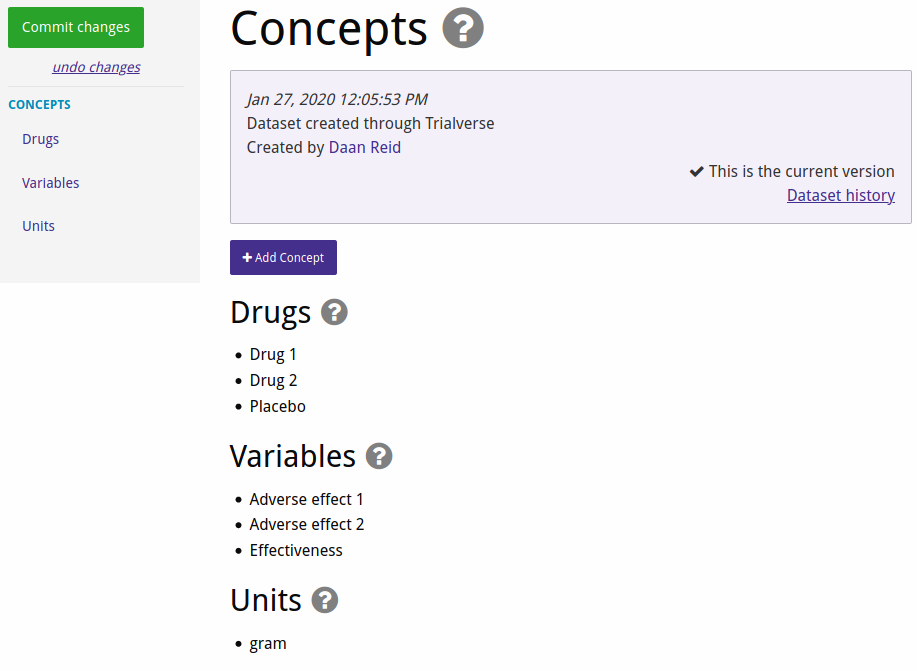
\includegraphics[width=0.7\textwidth]{img/concepts.png}
  \caption{Concept definitions for use in the dataset.}
\label{fig:concepts}
\end{figure}

The ADDIS study data repository has an audit trail, recording all changes and letting you use different versions of a dataset for analysis as desired.
New versions are created by explicitly committing changes to the database.

Once you've created the desired concepts, commit them using the green 'Commit changes' button at the top-left, entering a descriptive message such as 'create concepts.'
Navigate back to your dataset view by clicking its name in the breadcrumbs trail at the top of the page.

\textbf{As a general note, it is unfortunately wise before committing your work to open the ADDIS website in a separate tab to see whether you're still logged in, and if not, to log in again in this tab.
For security reasons, we log you out after a period of inactivity, and working on data without committing doesn't count at the moment.
We're working on ways to resolve this, and apologise for the inconvenience.}

\subsection{Entering a study}

After creating the concepts, it's time to create a study.

There are multiple ways to import data into ADDIS but for simplicity's sake in this tutorial we perform manual entry.

Click the '\textbf{+}' button next to the 'Studies' header, and create a new, empty study with a simple short title ('Study 1' will do) and a descriptive longer one (we intend to compare drug 1 with placebo in this one, so a longer title to that effect will be helpful).

Once the study is created, click on its title to navigate to the study interface.
First, we can indicate some meta-data about the study such as whether it was randomized, what the indication is and the eligibility criteria, but in this tutorial we're only creating a bare-bones study for analysis.
Scroll down to the 'Arms' section, and create two arms, titled 'Drug 1' and 'Placebo.' (Figure~\ref{fig:arms})

\begin{figure}[!ht]
  \centering
  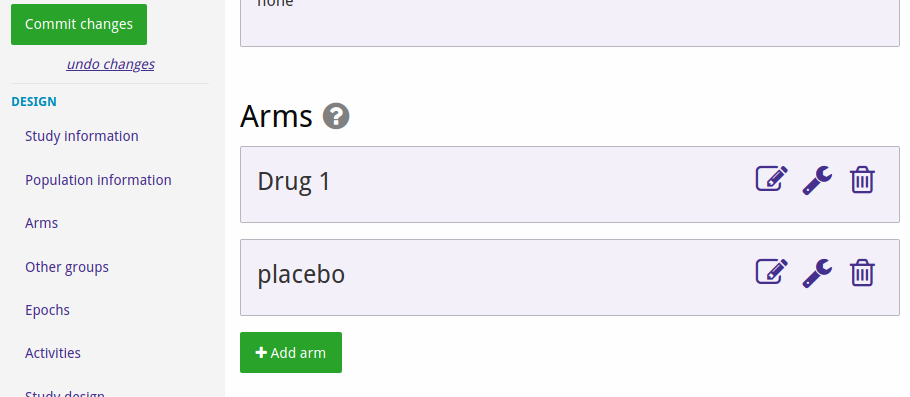
\includegraphics[width=0.7\textwidth]{img/arms.png}
  \caption{Arms for the first study.}
\label{fig:arms}
\end{figure}

After this, scroll down to the Epochs section, and create an epoch called 'Treatment phase'.
Set it to have a duration and choose a length (the value is not important for analytical purposes).
Be sure to check the 'primary epoch' checkmark - this indicates that this time period in the study is the one where primary treatment takes place (Figure~\ref{fig:createMainPhase}).
You can create more epochs, such as screening or randomization, but it's not necessary here.

\begin{figure}[!ht]
  \centering
  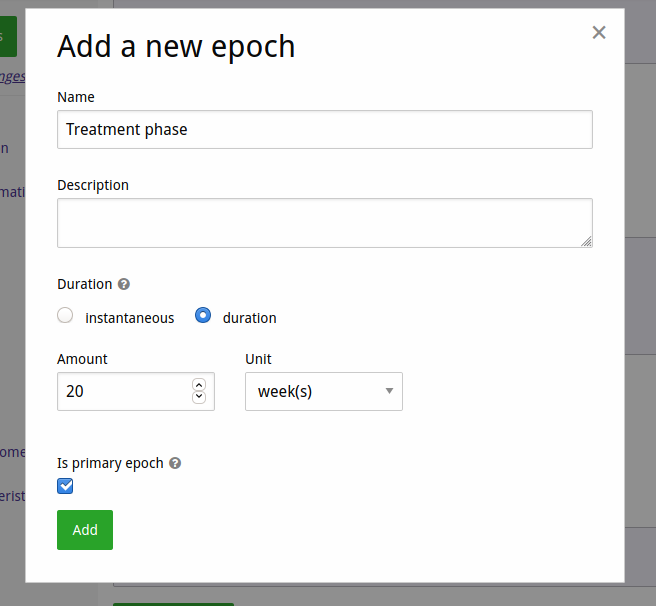
\includegraphics[width=0.7\textwidth]{img/createMainPhase.png}
  \caption{Creating the primary treatment epoch.}
\label{fig:createMainPhase}
\end{figure}

In the next section, create an activity of type 'drug treatment' for both 'Placebo' and 'Drug 1.'
Click the 'Add treatment drug' button to add a drug to the treatment activity in each case (Figure~\ref{fig:addPlaceboTreatment}).
Note that the name of the drug and the actual dosage are separately defined.
Use a dosage of 0 milligram per day for Placebo, and choose your own dosage for Drug 1.

\begin{figure}[!ht]
  \centering
  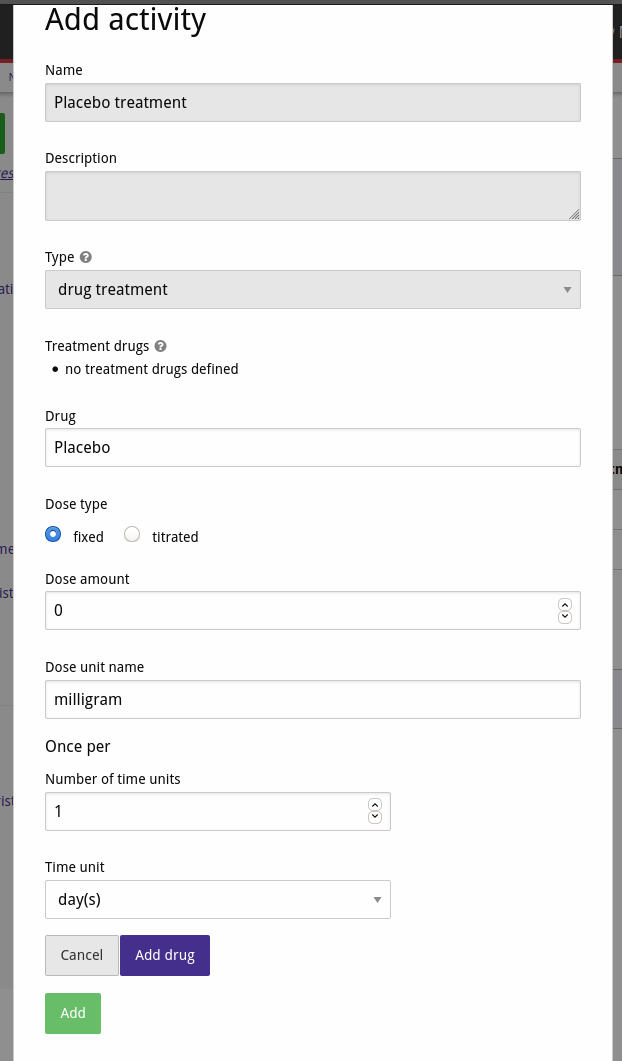
\includegraphics[width=0.7\textwidth]{img/addPlaceboTreatment.png}
  \caption{Creating the placebo treatment activity.}
\label{fig:addPlaceboTreatment}
\end{figure}

We can now combine the arms, epochs and activities to describe the study design in the next section.
Use the dropdowns in the study design table to assign the drug treatments to their appropriate arm.
In Figure~\ref{fig:studyDesign} you can see an example of a slightly more complex study design in which the randomization activity is performed in its own (instantaneous) epoch.

\begin{figure}[!ht]
  \centering
  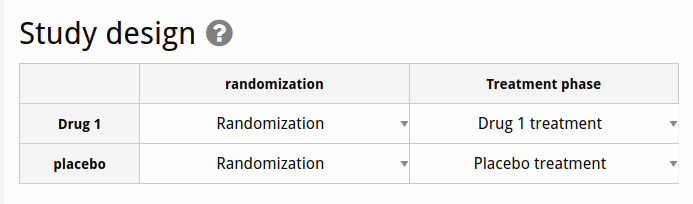
\includegraphics[width=0.7\textwidth]{img/studyDesign.png}
  \caption{Filling out the study design.
  Arms are rows and epochs are columns, and each cell contains an activity.}
\label{fig:studyDesign}
\end{figure}

We need to indicate when data were measured in the study.
We do so with measurement moments, which define a point anchored in the epoch structure we defined earlier.
Create a measurement moment in the next section, setting it to be at the end of the 'Treatment phase' epoch (Figure~\ref{fig:addMeasurementMoment}).

\begin{figure}[!ht]
  \centering
  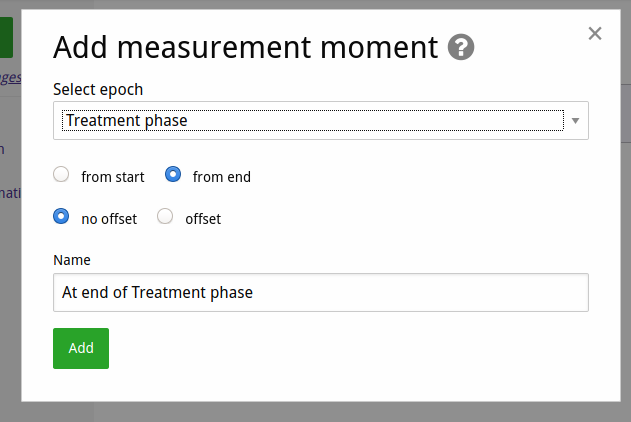
\includegraphics[width=0.7\textwidth]{img/addMeasurementMoment.png}
  \caption{Creating a measurement moment.}
\label{fig:addMeasurementMoment}
\end{figure}

Now everything is in place we can begin creating variables and reporting their measurements.
Create an Outcome called 'Effectiveness.'
Set its type to continuous and leave the included properties on their default values.
Be sure to indicate that the outcome is measured during the measurement moment you created earlier by checking its box (Figure~\ref{fig:effectiveness}).

\begin{figure}[!ht]
  \centering
  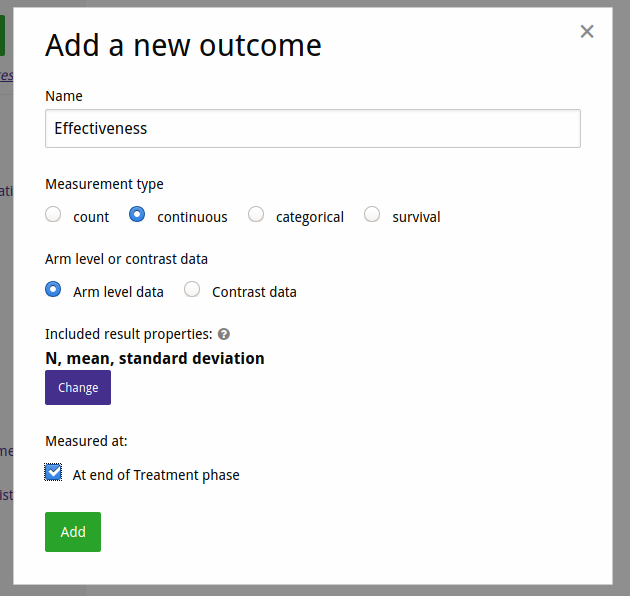
\includegraphics[width=0.7\textwidth]{img/effectiveness.png}
  \caption{Creating the effectiveness outcome.}
\label{fig:effectiveness}
\end{figure}

After creating the outcome, you can enter data for each of the measurement moments at which you've indicated it is measured.
Click the 'Show measurements' button to reveal the data table, and fill it out as shown in Figure~\ref{fig:measurements}.
Note that the actual values here aren't all that important, they have simply been chosen for demonstration purposes.

\begin{figure}[!ht]
  \centering
  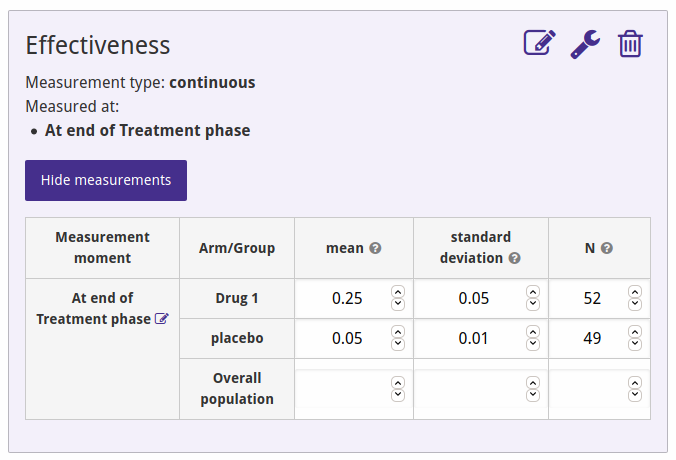
\includegraphics[width=0.7\textwidth]{img/measurements.png}
  \caption{Entering data for the effectiveness outcome.}
\label{fig:measurements}
\end{figure}

Now, create two adverse events, each of the 'count' type and fill out their data tables as well (Figure~\ref{fig:aeData}).

\begin{figure}[!ht]
  \centering
  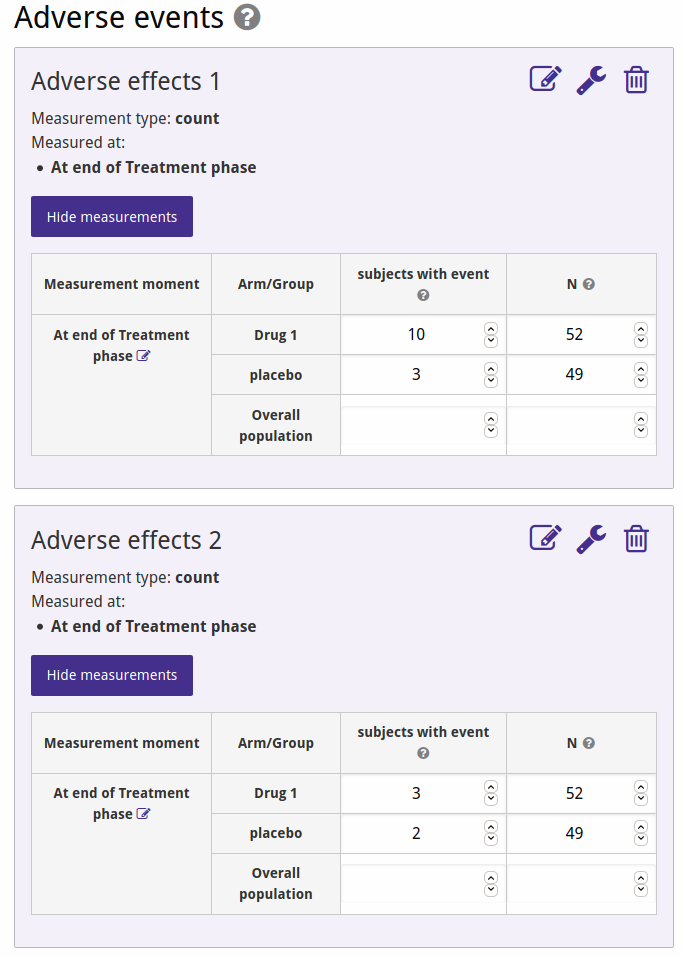
\includegraphics[width=0.7\textwidth]{img/aeData.png}
  \caption{Filling out the adverse events measurement tables.}
\label{fig:aeData}
\end{figure}

Finally, we need to indicate how the concepts within this study relate to the concepts as the dataset level.
We call this 'mapping' and it is performed in the 'Concepts mapping' section.
Please fill this out as shown in Figure~\ref{fig:conceptMappings}.
Note the way in which we map the milligram unit used in dosages here to the 'gram' concept at the dataset level by setting a multiplier prefix.
This makes harmonization between different units much easier.

\begin{figure}[!ht]
  \centering
  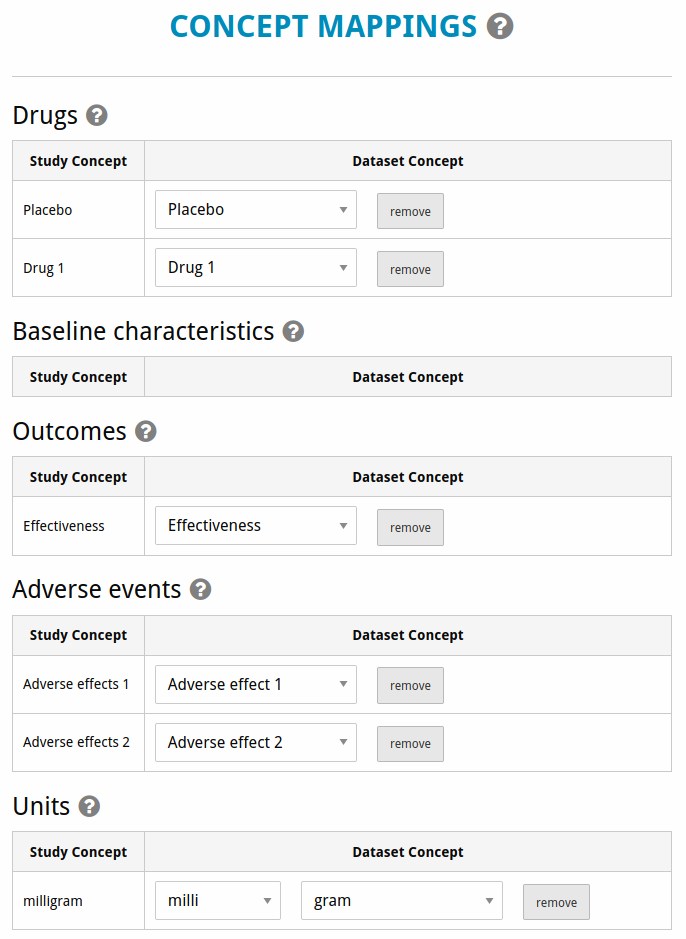
\includegraphics[width=0.7\textwidth]{img/conceptMappings.png}
  \caption{Mapping the concepts from study 1 to those of the dataset.}
\label{fig:conceptMappings}
\end{figure}

Now that you've mapped the concepts, entering this study is done.
Commit your work using the green 'Commit changes' button at the top left, again with an informative message such as 'entered Study 1.' Again, remember to check whether you're still logged in in a separate tab before committing.

\subsection{Copying a study}

Performing an indirect treatment comparison or network meta-analysis only really makes sense if you have at least two studies.
We've entered a second study into the demonstration dataset, so you don't have to do the work of entering that one as well.
Instead, you can copy it to your own dataset to reuse it.
Navigate to the \href{https://addis.drugis.org/#/users/12/datasets/c190e953-051c-4cf5-ac10-332984a14a43}{tutorial dataset}, click on 'Study 2' and then click on the 'Copy study' button at the top-right.
Select your own dataset as the target, and navigate there once the copy has finished (Figure~\ref{fig:copyStudy}).
Be sure to update the concept mappings in your newly-copied study to refer to the correct concepts in your dataset.

\begin{figure}[!ht]
  \centering
  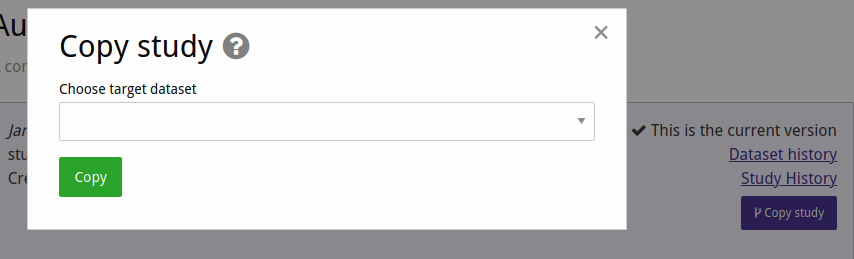
\includegraphics[width=0.7\textwidth]{img/copyStudy.png}
  \caption{Copying a study from one dataset to another.}
\label{fig:copyStudy}
\end{figure}

Now you have enough data to perform a simple network meta-analysis.

\section{Creating an analytical project}

Navigate to the dataset overview screen for your dataset, click the 'Create project' button at the top right, and create a new analytical project based on the dataset you just created.
Note that this button is also present when viewing other people's datasets -- analyses can be applied to data that you didn't enter.

First, we define which concepts (outcomes, interventions, units, covariates) from the dataset we wish to use in our analysis.
Click the 'Add outcome' button and select the Effectiveness semantic outcome from those available.
In this case, higher values are better.
Do the same for Adverse event 1 and 2, but indicate that lower is better there.

Next, click 'Add intervention' (Figure~\ref{fig:addIntervention}).

\begin{figure}[!ht]
  \centering
  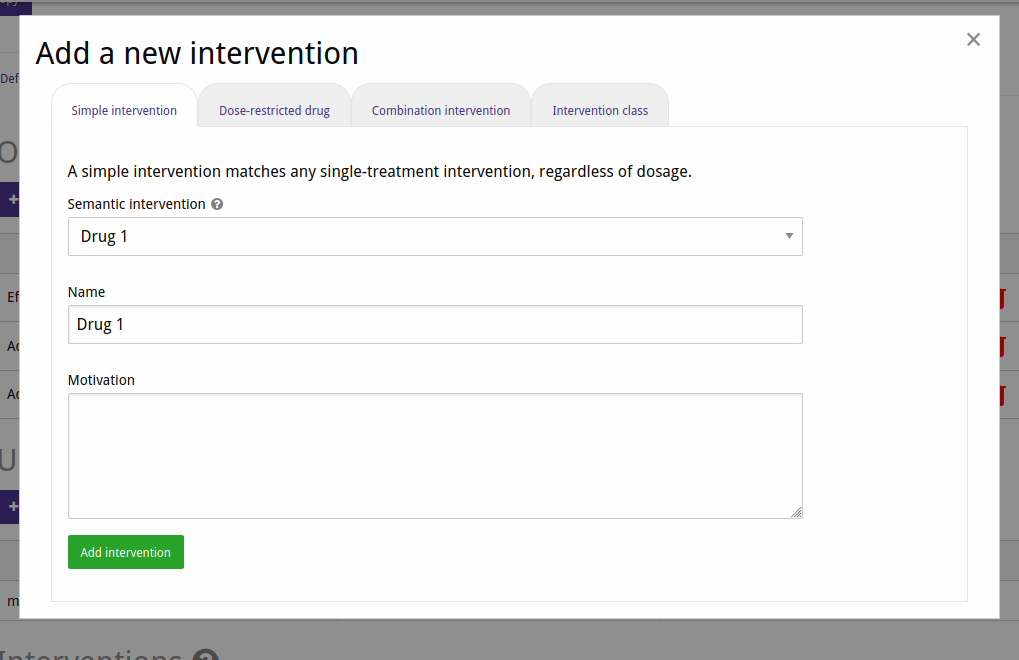
\includegraphics[width=0.7\textwidth]{img/addIntervention.png}
  \caption{Creating an evidence network.}
\label{fig:addIntervention}
\end{figure}

Note the tabs which allow for precise definitions concerning dosage restrictions, combination therapies and equivalence classes between specific interventions.
Here, we'll stick to simple interventions.
Create a simple intervention for Placebo, Drug 1 and Drug 2.
We won't be showing covariates or more complex intervention definitions (which require units for the dosage) in this tutorial so this is enough to start our analysis.

\section{Performing evidence synthesis}

Go to the 'Analyses' tab and click the 'Add analysis' button.
Create an evidence synthesis, and call it something like 'Effectiveness network.'
On the following network creation screen, select the outcome of interest (Effectiveness), and select all interventions one by one.
Notice how the evidence network and table are automatically updated as your selections change  (Figure~\ref{fig:createNetwork}).

\begin{figure}[!ht]
  \centering
  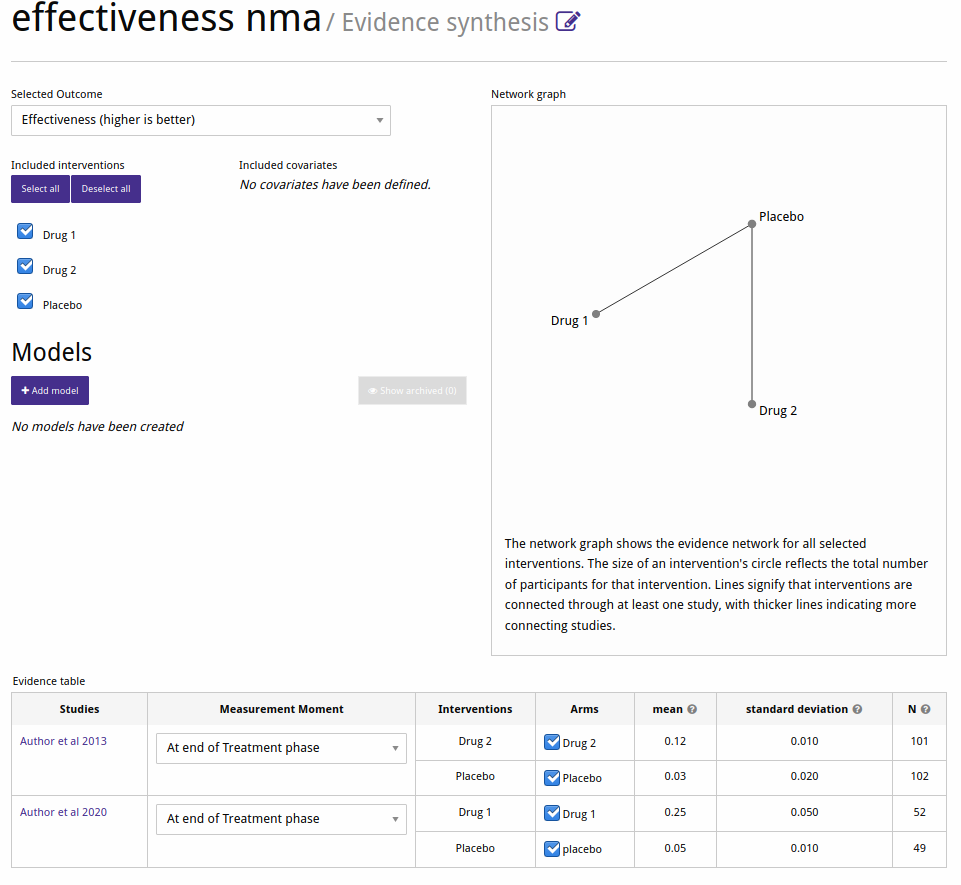
\includegraphics[width=0.7\textwidth]{img/createNetwork.png}
  \caption{Creating an evidence network.}
\label{fig:createNetwork}
\end{figure}

In the network diagram you can see which interventions are directly compared in at least one study: they are connected with a line.
The lines get thicker as more studies compare those two interventions; the circles get larger as the total sample size for that intervention increases.
You can override the automatic evidence selection by unchecking specific arms in the evidence table, or by changing which measurement moment's data will be used.

Once you are satisfied with your evidence network, click the 'Add model' button and take some time to look at the available model creation options if you are interested.
Unfortunately, explaining them goes beyond the scope of this tutorial.
Please see the \href{https://addis.drugis.org/manual.html#model-creation}{ADDIS manual} for more details.
The default model is a random-effects consistency model, which is fine for now.
Please enter a descriptive model title (e.g. 'RE consistency') and create the model.
After brief computation, you will see the model results.
Again, a full explanation of the results is beyond the scope of this tutorial.
One of the main outputs of a network consistency model is the relative effects table (Figure~\ref{fig:relativeEffects}), which shows how much stronger the effect in question is for each individual comparison between treatments in the network (including indirect ones).

\begin{figure}[!ht]
  \centering
  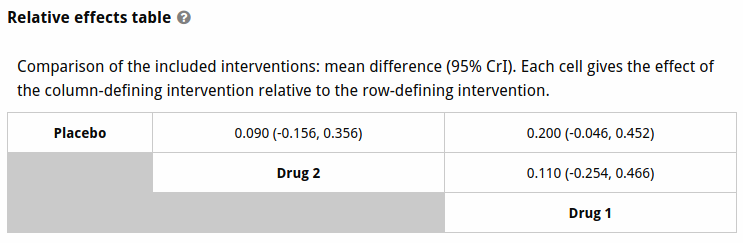
\includegraphics[width=0.7\textwidth]{img/relativeEffects.png}
  \caption{The relative effects in the evidence network.}
\label{fig:relativeEffects}
\end{figure}

\section{Updating evidence and analyses}

One of the strengths of ADDIS is that when new evidence comes to light or mistakes are fixed, analytical projects can be automatically updated when their source dataset changes.
Navigate to the \href{https://addis.drugis.org/#/users/12/datasets/c190e953-051c-4cf5-ac10-332984a14a43}{tutorial dataset} and copy Study 3 (a three-arm study introducing a new drug) to your dataset.
Now click on the 'Projects' tab and go to your analytical project.
Note that there is now a warning indicating that your project is based on an older version of the dataset (Figure~\ref{fig:updateWarning}).

\begin{figure}[!ht]
  \centering
  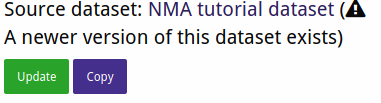
\includegraphics[width=0.7\textwidth]{img/updateWarning.png}
  \caption{A warning indicating that the source dataset of an analytical project has updated.}
\label{fig:updateWarning}
\end{figure}

Of course this is fine in many cases, but if you know that you want to include the changes in your analyses, you can click the 'Update' button.
Take a moment to read the explanation of what will happen.
Most importantly, your old analysis will not be lost, but simply archived (i.e. hidden by default).
You can undo the archiving operation.

Confirm the update, click 'Add intervention' and add a new intervention for Drug 3.
Navigate to the 'Analyses' tab and click on your evidence synthesis. 
Note that your model has not been updated, but instead there is none.
The assumption here is that if the possibilities of evidence networks change, users would prefer to recreate their models with the new evidence.
Add 'Drug 3' to the selected interventions and again create a relative effects consistency model.
Take a moment to explore the new results. 

\section{Conclusion}

This concludes the tutorial.
You've entered your own study data, copied some from another user, and defined and performed a network meta-analysis based on these data.
You've also updated your analyses when new evidence came to light.
Thank you very much for your time.
We hope this was clear and educational.
Please don't hesitate to contact the author with feedback.

\end{document}
